\section{Search in the All-Hadronic Final State}
\label{sec:alphat}

\begin{figure*}[!ht]
\centering
%\begin{center}
\begin{tabular}{cc}
\subfloat[] {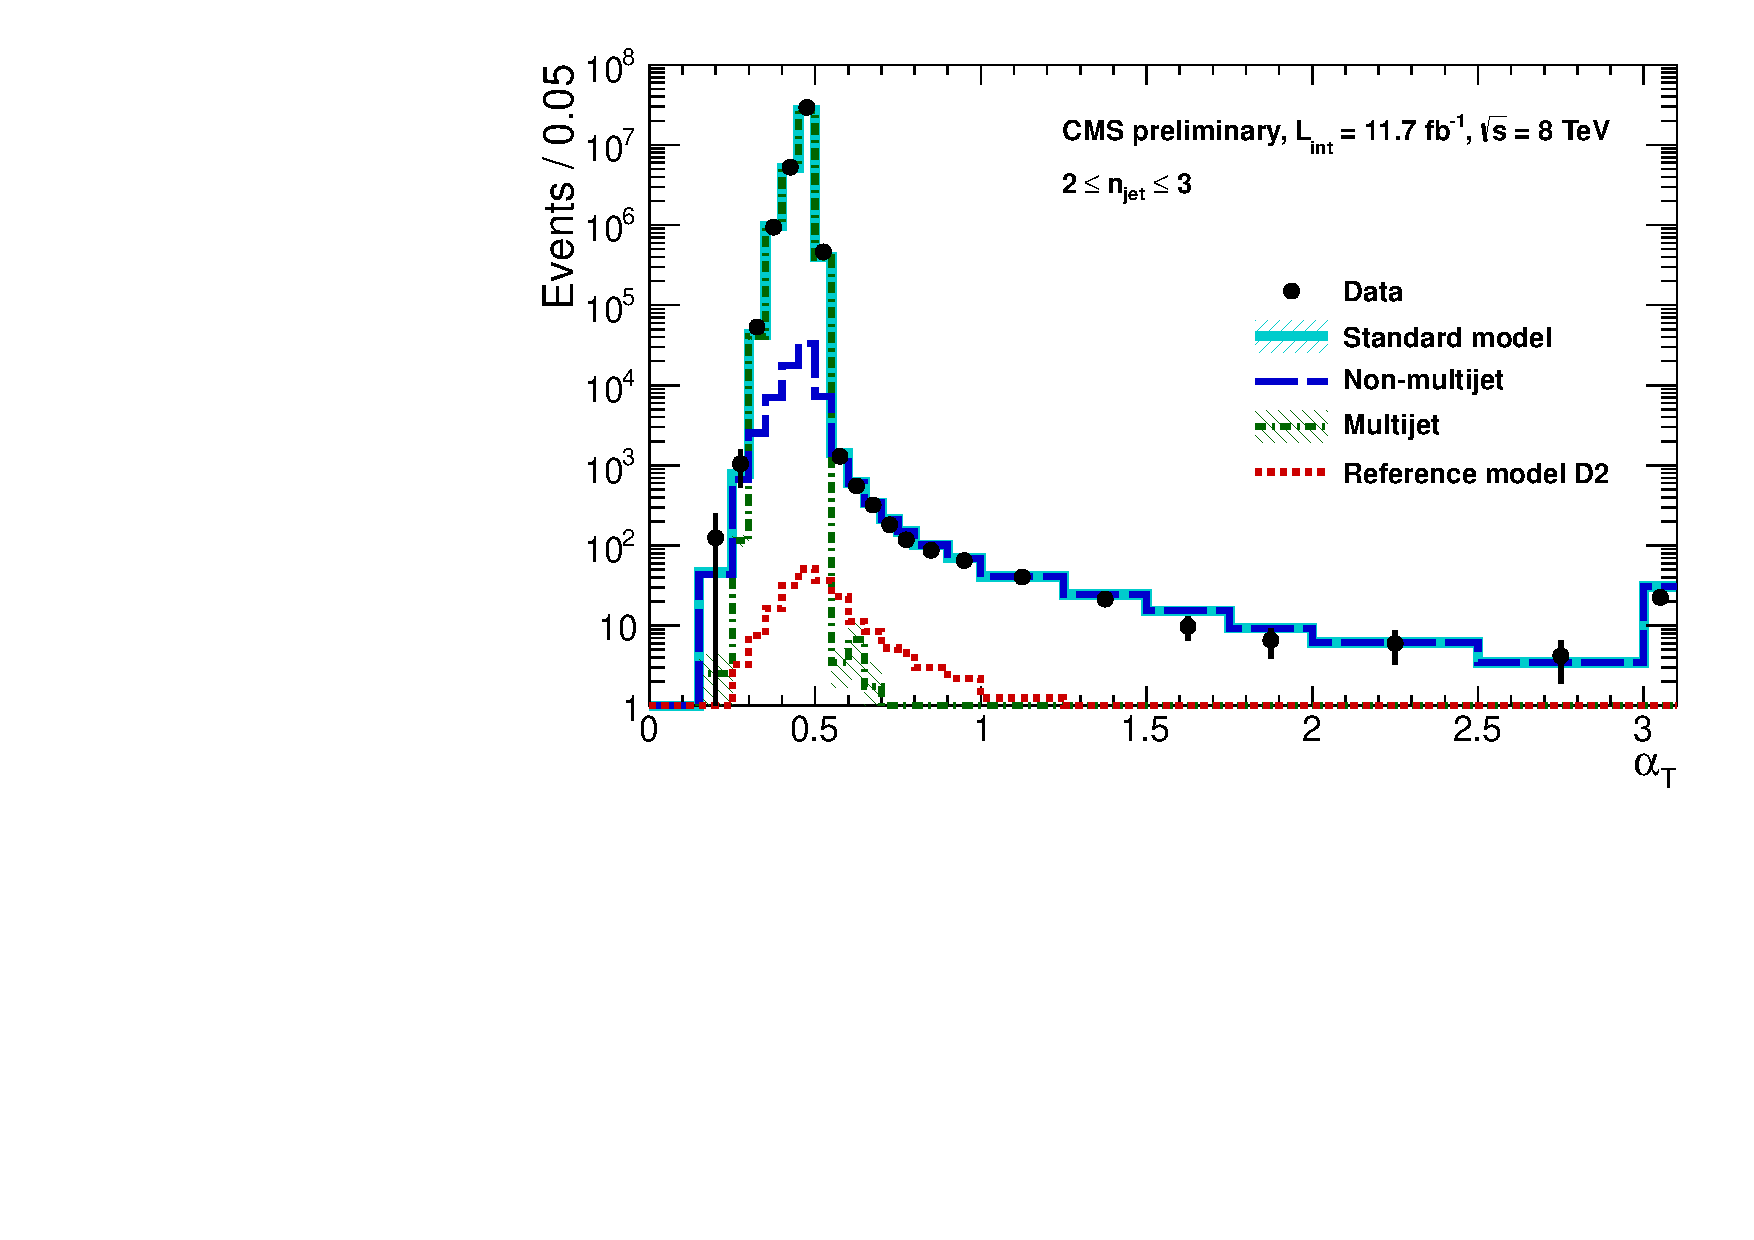
\includegraphics[width=0.45\textwidth]{HCPPlots/AlphaT_le3j_prelim.pdf}} &
\subfloat[] {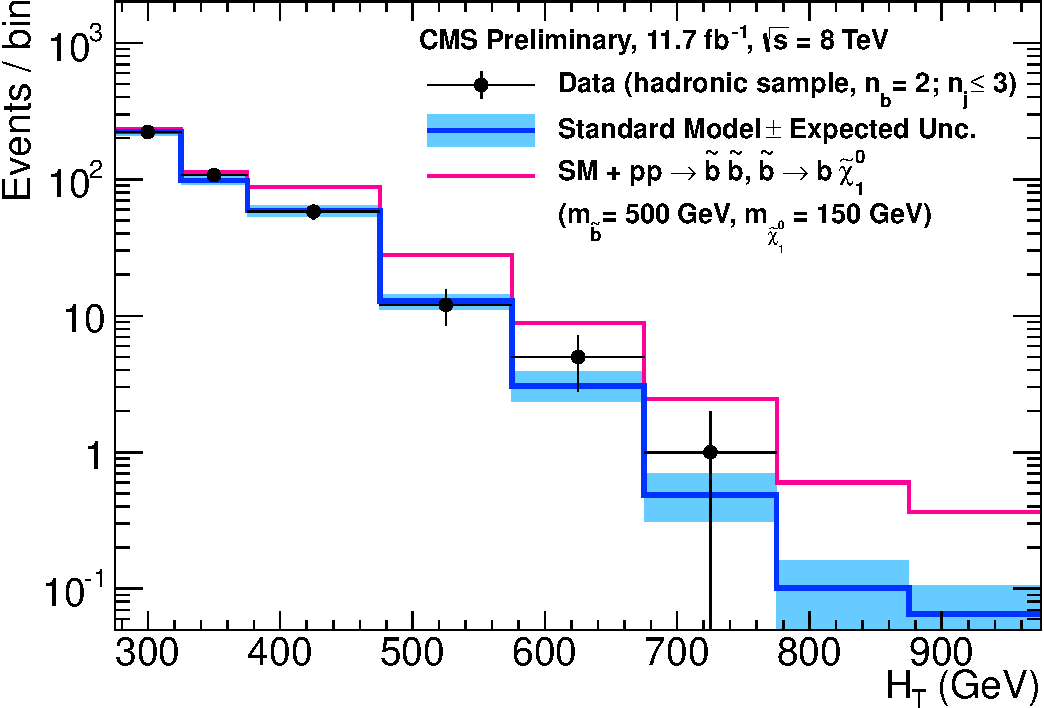
\includegraphics[width=0.4\textwidth]{HCPPlots/hadronic_2b_le3j_logy.pdf}} \\
\end{tabular}
\caption{
The distribution of the \alphat\ variable (left) and the $H_T$ distribution in data, compared to the SM background expectation (right).
\label{fig:alphat}
}
%\end{center}
\end{figure*}

The production of bottom squark pairs, followed by the decay $\tilde{b}\to b\lsp$, leads to events with
two b-jets and \met. In this section we report the results from a search with 11.7 fb$^{-1}$ 
in the all-hadronic final state using the 
\alphat\ variable.%, discussed below, which discriminates between backgrounds with real and fake \met.

We count jets with \pt\ $>$ 50 GeV. The leading (highest \pt) jet is required to be in the tracker 
acceptance defined by $|\eta|<2.5$, and the leading two jets must satisfy \pt\ $>$ 100 GeV. Events with isolated 
electrons or muons with \pt\ $>$ 10 GeV are vetoed, in order to suppress backgrounds with neutrinos from the decays 
of W bosons. Events with an isolated photon with \pt\ $>$ 25 GeV are vetoed.
The remaining events are categorized based on the jet multiplicity, the number of b-tagged jets (using CSVM) and the event $H_T$, 
which is required to satisfy $H_T$ $>$ 275 GeV.

The background satisfying the above preselection is dominated by QCD multijet production with fake \met\ from mismeasurement effects. To suppress this background,
we make requirements on the quantity $\alphat$. For dijet events this quantity is defined as $\alphat \equiv E_{T}^{j_2} / M_{T}$, where $E_{T}^{j_2}$ is the $E_T$
of the second leading jet and $M_T$ is the transverse mass of the dijet system. 
For events with perfectly measured jets, the measured \pt\ values of the two jets are equal, leading to $\alphat=0.5$. The key feature of the \alphat\ variable
is that mismeasurement effects tend to decrease the value of \alphat, such that it is extremely rare for events with fake \met\ to have \alphat\
much larger than 0.5. As shown in Fig.~\ref{fig:alphat}(a), the \alphat\ distribution for the QCD multijet background falls off extremely rapidly near this endpoint value.
For events with three of more jets, an equivalent dijet system is formed by  clustering the jets into two pseudo-jets. In our search we strongly suppress the
QCD multijet background with the requirement \alphat\ $>$ 0.55.

The background after the \alphat\ requirement is dominated by processes with genuine \met, including \ttljets\ and \wjets\ with a lepton and neutrino from W decay,
where the lepton is either not reconstructed or is a hadronically decaying $\tau$ lepton. 
These backgrounds are estimated using a $\mu+\rm{jets}$ data control sample.
The additional background from $\rm{Z}(\nu\nu)+\rm{jets}$ is estimated using two data control samples of $\rm{Z}(\ell\ell)+\rm{jets}$ and  $\gamma+\rm{jets}$ events. To estimate these backgrounds, the observed yields in the data control samples are extrapolated to the
signal region using translation factors derived from MC. The dominant systematic uncertainties in the background prediction stem from the uncertainties
in the MC translation factors, which are assessed by performing several closure tests in data. In these tests, the observed yields in one data control region
are used to predict the yields in another data control region.

Events are categorized based on the $H_T$, jet multiplicity, and b-tagged jet multiplicity. For the bottom squark scenario described above, the most sensitive
category is events with either two or three jets and exactly two b-tagged jets. The $H_T$ distribution for these events is indicated in Fig.~\ref{fig:alphat}(b),
which demonstrates good agreement between the data and the expected background. No evidence for an excess of events is observed.

The results are interpreted  using the model of bottom squark pair production with $\tilde{b}\to b\lsp$ in Fig.~\ref{fig:ss_interpretation}(b).
These results probe bottom squarks with masses up to approximately 600 GeV. Additional interpretations in models with gluino-mediated
top and bottom squark pair production are presented in Ref.~\cite{ref:alphat}.

